\label{sec:cronograma}

A \autoref{fig:crono} exibe o cronograma proposto para a próxima etapa do trabalho de conclusão de curso, essas atividades são:

  \begin{description}  
  \item[Revisão da literatura sobre invariantes de memória:] Invariantes de memória adicionam condições de pré e pós execução de operações sobre memória, sendo importante para 
  este trabalho no que concerne a geração de \textit{witness}; 
  %
  \item[Aprimoramento do rastreamento de memória:] Comparar o rastreamento memória atual em outros modelos de memória, exemplo, o de precisão de \textit{bit} utilizado pelo VALGRING;
  %
  \item[Definição formal das propriedades de memória utilizado na verificação:] Criação de regras lógicas (baseada na lógica de inferência de Hoare \cite{Rocha:2015tese}) para as propriedades verificadas pelo Map2Check. 
  %
  \item[Aplicação de um \textit{slicer} de código para o Map2Check:] No modelo atual, a instrumentação do Klee pode gerar muitos casos e facilmente gerar um número excessivo de estados, assim como o Symbtiotic 3 \cite{Chalupa:2016} vamos utilizar um \textit{slicer} pra resolver esse problema.
  %
  \item[Adicionar \textit{bounded model checker} no método:] Com o uso de BMC será possível gerar outras propriedades de segurança de memória de forma mais otimizada, devido a aplicação de outras técnicas como \textit{Lazy Abstraction} \cite{Cordeiro:2012}
  %
  \item[Tradução das propriedades do \textit{bounded model checker}:] É necessário fazer com que o Map2Check seja compatível com a propriedades geradas pelo BMC, logo serão traduzidas as propriedades.
  %
  \item[Avaliação experimental das novas propriedades suportadas pelo método:] Testes empíricos sobre as novas funcionalidades.
  %
  \item[Realização de experimentos com \textit{benchmarks} públicos de programas escritos em C:] Com esses experimentos podemos verificar a eficácia real do método.
  %
  \item[Escrita de artigos:] Escrita de artigos para divulgação dos resultados do método.
  %
  \item[Finalização da monografia:] Escrita sobre tudo o que foi desenvolvido e estudado no trabalho.
  %
  \item[Apresentação final:] Defesa do trabalho de conclusão de curso.
\end{description}


\begin{table}[H]
	\caption{\label{fig:crono} Cronograma do projeto}
	\begin{center}
	    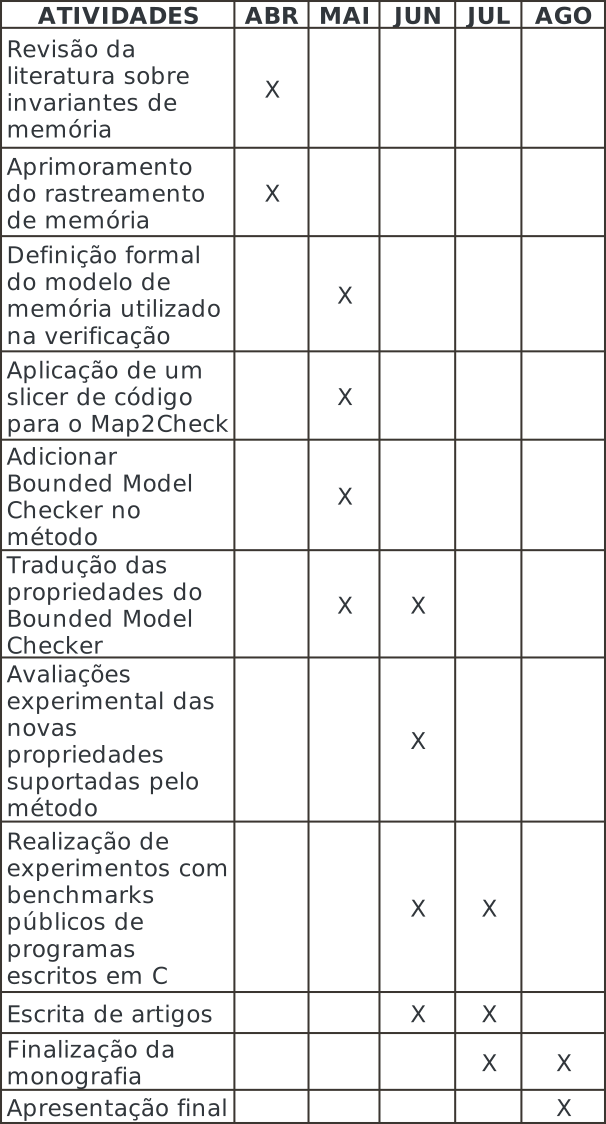
\includegraphics[scale=0.75]{resources/crono.png}
	\end{center}
	\legend{Fonte: Própria}
\end{table}

\newpage